% %%%%%%%%%%%%%%%%%%%%%%%%%%%%%%%%%%%%%%%%%%%%%%%%%%%%%%% %
% Template File for LateX                                 %
% Christoph Glanzer, Stephan Artmann                      %
% christoph.glanzer@ifor.math.ethz.ch                     %
% stephan.artmann@ifor.math.ethz.ch                       %
% %%%%%%%%%%%%%%%%%%%%%%%%%%%%%%%%%%%%%%%%%%%%%%%%%%%%%%% %

\documentclass[sigconf]{acmart}

% Packages used
\usepackage[utf8]{inputenc}
\usepackage{amsmath, amsbsy, amsthm}
\usepackage{enumerate} % To enumerate with roman numbers
\usepackage{datetime} % \currenttime

\setcopyright{none}
\settopmatter{printacmref=false,printfolios=false}
\renewcommand\footnotetextcopyrightpermission[1]{} % removes footnote with conference information in first column
\pagestyle{plain} % removes running headers

\setlength{\parindent}{0pt} % To avoid margins.

\title{Recognizing Italian Sign Gestures with Bidirectional\\Neural Networks}
\author{Stephan Artmann{\normalsize${}^{\ast}$} and Christoph Glanzer}
\authornote{Authors are listed in alphabetical order as they contributed equally.}
% %%%%%%%%%%%%%% %
% Extra Commands %
% %%%%%%%%%%%%%% %

\newcommand{\Z}{\mathbb{Z}}
\newcommand{\R}{\mathbb{R}}
\newcommand{\Q}{\mathbb{Q}}
\newcommand{\N}{\mathbb{N}}
\newcommand{\inv}{^{-1}}
\newcommand{\invtransp}{^{-T}}
\newcommand{\spann}{\text{span}}
\newcommand{\lattice}{\mathcal{L}}
\newcommand{\hnf}{\texttt{HNF}\xspace}
\newcommand{\tu}{\texttt{TU}\xspace}
\def\T{^\mathrm{T}}
\newcommand{\quotmarks}[1]{``#1''}
\newcommand{\nth}[2]{\ensuremath{{#1}^{\text{\tiny{#2}}}}\xspace}

\def\conv{\operatorname{conv}}
\def\aff{\operatorname{aff}}
\def\st{\operatorname{ s.t. }}
\def\lin{\operatorname{lin}}
\def\dom{\operatorname{dom}}
\def\int{\operatorname{int}}
\def\relint{\operatorname{relint}}
\def\rec{\operatorname{rec}}

\def\cone{\operatorname{cone}}
\def\vol{\operatorname{vol}}

% Change enumeration sign
%\def\labelitemi{\tiny$\blacksquare$}
\def\labelitemi{\raisebox{1pt}{\scalebox{0.45}{$\blacksquare$}}}

% %%%%%%%%%%%%% %
% Main Document %
% %%%%%%%%%%%%% %

\begin{abstract}
	During a project at ETH Zürich, we have implemented a neural network in TensorFlow which recognizes Italian sign gestures from short video clips. Using a bidirectional neural network architecture we were able to beat the \emph{hard}-baseline with our model, reaching a correct classification rate of 82.8\% on test data.\\
	
	This report will give a detailed description of our model architecture. \textit{Unfortunately, for reasons of copyright, we are unable to publish most of our code in this repository.}
\end{abstract}

\begin{document}
	\maketitle
	
	\section{Description of the task}
	The data is a modified version of the \href{http://chalearnlap.cvc.uab.es/dataset/13/description/}{\textit{ChaLearn Multimodal Gesture Recognition dataset}}. Each sample consists of a video clip, depth data, a segmentation mask, and skeletal information (cf. Figure~\ref{fig:sample}). Data is provided in the TFRecord file format. The resolution of the video clip, depth information and the segmentation mask is $80 \times 80$ pixels per frame. The video clips are of different length. The goal is to correctly classify 20 different sign gestures.
	\begin{figure}[h!]
		\begin{center}
			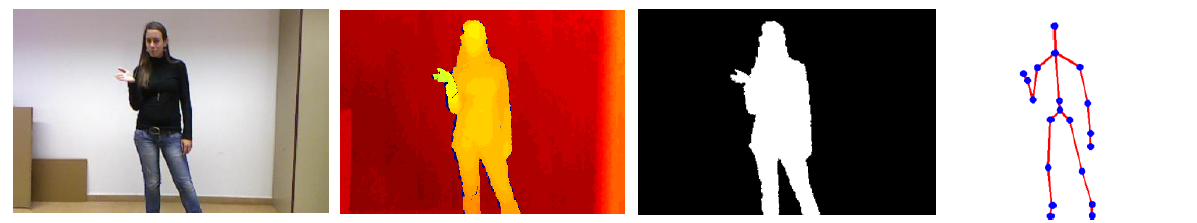
\includegraphics[width=0.5\textwidth,height=0.5\textheight,keepaspectratio]{sample.png}
		\end{center}
		\caption{Sample frame from a video clip. The data includes depth data, a segmentation mask, and skeletal information (Image source: \href{http://chalearnlap.cvc.uab.es/dataset/13/description/}{Sergio Escalera, Computer Vision Center and University of Barcelona}).}
		\label{fig:sample}
	\end{figure}
	
	\section{Overview}
	The architecture of our model is based on the work of Pigou et al. \cite{pigou}. The model we took as a baseline is the bidirectional CNN-RNN depicted in Figure~\ref{fig:model}.
	
	\begin{figure}[h!]
		\begin{center}
			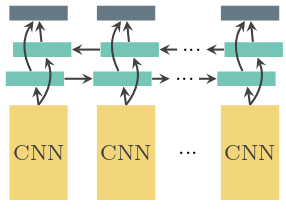
\includegraphics[width=0.2\textwidth,height=0.2\textheight,keepaspectratio]{model.png}
		\end{center}
		\caption{The bidirectional CNN-RNN which forms the basis of our model, cf.~\citep[Figure 1c]{pigou}.}
		\label{fig:model}
	\end{figure}
	
	Due to the fact that Pigou et al. have a different, higher-resolution dataset and as a consequence of our observations, we have modified this model quite significantly. The three main ideas which we borrow from this architecture are the bidirectional setup, the design of the CNN in which two convolutional layers are stacked before performing a max-pooling step and the regularization techniques employed. However, we did not implement the peephole connections visible in Figure~\ref{fig:model} as we observed that one bidirectional layer was sufficient. Furthermore, our model has a significantly lower number of variables, especially due to smaller dense layers.
	
	One of the main challenges of this project is the prevention of overfitting. We have achieved this by implementing various regularization techniques which we will describe in detail below. Furthermore, we have identified some invalid (wrongly clipped) videos in the training data, cf. Section~\ref{sct:5}.\footnote{We wish to emphasize that our data is a modified version of the \href{http://chalearnlap.cvc.uab.es/dataset/13/description/}{\textit{original ChaLearn dataset}}.}
	
	\section{Detailed Model Architecture}
	
	The data is fed into the model in batches of $8$ videos each.\footnote{The small batch-size is due to memory limitations on the GPU.} Every frame of each video is fed into a convolutional neural network. This CNN admits shared weights, i.e., every frame is fed into the same CNN. The architecture of the CNN is depicted in Figure~\ref{fig:our_model}. The filter size of each convolutional layer is $3x3$, where we use same padding. We use leaky ReLUs after each convolutional layer with a value of $\alpha = 0.3$. The max-pooling layers use a pooling size of $2x2$ and a striding of $2$ in each direction. The output is fed into a dropout layer ($p=0.5$) and subsequently into a dense layer, which again uses leaky ReLUs with $\alpha = 0.3$. The latter has an output size of $128$ units.\footnote{When using two dense layers of $2048$ units each as suggested in~\cite{pigou}, we obtained significantly worse results. We assume that this stems from the fact that the dataset used in their paper has a higher resolution.}\\
	
	Next, we feed the output of the CNN into a bidirectional neural network with one layer. We employ long short-term memory units~\cite{lstm} with $256$ hidden, resp. output units. The output is fed into a dropout layer $(p = 0.5)$ and a dense layer (leaky ReLUs, $\alpha = 0.3$) with an output size of $20$ units generating the logit values. The loss is calculated as an average across all video frames. The model's prediction of the gesture label is the $\mathrm{argmax}$ of the average across all frames.
	
	\begin{figure}[h!]
		\begin{center}
			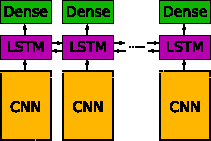
\includegraphics[width=0.25\textwidth,height=0.25\textheight,keepaspectratio]{rnn.pdf}
		\end{center}
		\caption{Graphical representation of our model.}
		\label{fig:rnn}
	\end{figure}
	
	\begin{figure}[h!]
		\begin{center}
			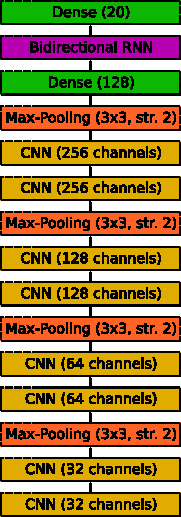
\includegraphics[width=0.5\textwidth,height=0.5\textheight,keepaspectratio]{our_model.pdf}
		\end{center}
		\caption{Graphical representation of the convolutional architecture of our model.}
		\label{fig:our_model}
	\end{figure}

	\section{Modalities employed}
	The data consists of RGB, depth, segmentation and skeletal data. The skeletal data is stored as coordinates of the joints. In a preprocessing step of the data, we convert the skeletal data into RGB images, where the joint locations are stored as red dots and the connections between those joints are stored as blue lines. Furthermore, to make use of the segmentation data, we multiply it with the RGB, resp. depth modality to 'cut out' the person visible in the video. This ensures that no unnecessary data is fed to the model. We then feed data consisting of $7$ channels to the model: The first three channels are the cut-out RGB data.  Channel four is the cut-out depth data. The last three channels contain the skeletal data as RGB image.\\
	
	Figure~\ref{fig:modalities} below was generated with a debugging script. The first row of images shows the normalized and regularized RGB, depth and segmentation data. The second row of images shows the corresponding cut-out RGB and depth data as well as the skeletal information.
	
	\begin{figure}[h!]
		\begin{center}
			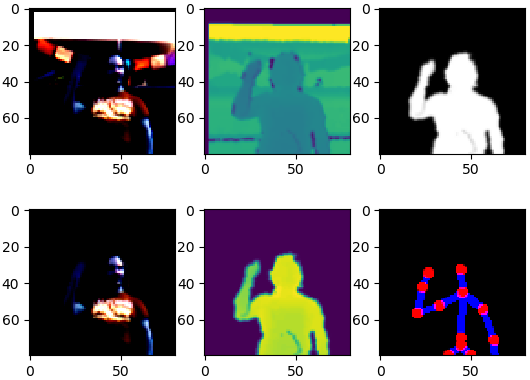
\includegraphics[width=0.45\textwidth,height=0.45\textheight,keepaspectratio]{modalities.png}
		\end{center}
		\caption{Modalities used in our model.}
		\label{fig:modalities}
	\end{figure}
	
	\section{Regularization}\label{sct:5}
	The main challenge of this project is to lower the generalization error. To this end, we have implemented the following regularization techniques, some of which are also used by~\cite{pigou}.
	
	\begin{itemize}
		\item Cropping: It turns out that many videos are badly cut and still contain gestures from the previous or next clip. Furthermore, the gestures are not always in the approximate middle of the video. To make up for this, we randomly crop up to 5 frames from the beginning and from the end of the video.\footnote{Cutting off more than 5 frames from the beginning / end decreases the test accuracy.}
		\item Random rotation of each video by $[-\pi/16,\pi/16]$ radians.
		\item Random translation of each video by $[-10,10]$ pixels horizontally and $[-5,5]$ pixels vertically.
		\item Randomly changing the brightness of each video by up to $30$\%.
		\item Resizing each video to a size of $82$\%-$118$\%.
		\item Dropout with $p=0.5$ before each Dense layer.
		\item Usage of leaky ReLUs with $\alpha = 0.3$ in the CNN and dense layers.
	\end{itemize}

	We observed that performing $L_2$-regularization does not improve the results. Furthermore, flipping does not improve the results. We believe that the latter is due to the fact that many gestures are already performed in a 'flipped' manner.\\
	
	\textbf{Early stopping:} We have created a python script that converts the data to .gif files. It turns out that the quality of the validation data is significantly worse compared to the training or test data. Many clips contain multiple gestures or badly recognizable gestures. This matches our observations: When training on both the training and validation data, the results are surprisingly worse (by 1-2\%)! Therefore, we have not implemented early stopping in our final submission.
	
%	\section{Contributions}
%	All contributions to this projects are from the team members only, with the exceptions of some ideas and models from \cite{pigou}, as stated in the previous sections.
	
	\bibliographystyle{ACM-Reference-Format}
	\bibliography{bibliography}
	
\end{document}